% This is samplepaper.tex, a sample chapter demonstrating the
% LLNCS macro package for Springer Computer Science proceedings;
% Version 2.20 of 2017/10/04
%
\documentclass[runningheads]{llncs}
%
\usepackage{booktabs}
\usepackage{graphicx}
\usepackage{pgfplots}
\usepackage{tikz}
\usepackage{enumitem}
\usepackage{gensymb}
\usepackage{amsmath}
\usepgfplotslibrary{clickable}

\newcommand{\Iris}{\ensuremath{\mathbf{I}}}
\newcommand{\Lits}{\ensuremath{\mathbf{L}}}
\newcommand{\Bnodes}{\ensuremath{\mathbf{B}}}
\newcommand{\Vars}{\ensuremath{\mathbf{V}}}

\newcommand{\da}{\ensuremath{:\nolinebreak\mkern-1.2mu\nolinebreak=}}

\newcommand{\ah}[1]{{\color{blue}\textsc{ah:} #1}}

\usepackage{xcolor}
\usepackage{hyperref}
\definecolor{dark-blue}{rgb}{0.0,0.0,0.2}
\definecolor{dark-green}{rgb}{0.0,0.2,0.0}
\definecolor{dark-red}{rgb}{0.2,0.0,0.0}
\hypersetup{
    colorlinks, linkcolor={dark-red},
    citecolor={dark-green}, urlcolor={dark-blue},
    pdftitle={Estimating the dynamics of SPARQL query results over Wikidata},    % title
    pdfauthor={Alberto Moya, Aidan Hogan},     % author
    pdfsubject={KGSWC 2019},   % subject of the document
    pdfkeywords={SPARQL;} {Linked Data;} {Dynamics;} {Wikidata;}, % list of keywords
}



\usepackage{listings}
\lstset{language=SQL,morekeywords={PREFIX,java,rdf,rdfs,url}}
% Used for displaying a sample figure. If possible, figure files should
% be included in EPS format.
%
% If you use the hyperref package, please uncomment the following line
% to display URLs in blue roman font according to Springer's eBook style:
% \renewcommand\UrlFont{\color{blue}\rmfamily}

\begin{document}
%
\title{Estimating the dynamics of\\SPARQL query results over Wikidata\thanks{This work was supported by CONICYT PFCHA, Doctorado Becas Chile/2017 -- 72180000, the Millennium Institute for Foundational Research on Data (IMFD) and FONDECYT Grant No. 1181896.}}
%
%\titlerunning{Abbreviated paper title}
% If the paper title is too long for the running head, you can set
% an abbreviated paper title here
%
\author{Alberto Moya \and
Aidan Hogan\orcidID{0000-0001-9482-1982}}
%
\authorrunning{A. Moya and A. Hogan}
% First names are abbreviated in the running head.
% If there are more than two authors, 'et al.' is used.
%
\institute{IMFD; DCC, University of Chile\\
\email{\{amoya,ahogan\}@dcc.uhile.cl}}
%
\maketitle              % typeset the header of the contribution
%
\begin{abstract}
In this work, we tackle the problem of estimating future changes in SPARQL query results over dynamic datasets; such work has applications for caching and remote synchronization. Our proposal is based on syntactic query features and (optionally) knowledge of the dynamics of predicates in the underlying dataset; the resulting model can be used to predict (1) whether or not the results for a query will change in the near future using classifiers, and (2) when they might change (if at all) using linear regression. To evaluate our proposal, we select Wikidata as our dataset and build a curated collection of real-world SPARQL queries. Our results show that the accuracy of the predictions of our proposed model is competitive with that obtained using knowledge of the complete historical evolution of the query results but at a lower cost.

\keywords{SPARQL \and Linked Data \and Dynamics \and Wikidata}
\end{abstract}
%
%
	%
\section{Introduction}
\label{sec:intro}
%
Many applications that consume Linked Data (LD) face challenges related to remote changes in the underlying data. Client-side caches can reduce the network traffic between clients and servers, the load on servers, and the average latency of responses. However, since datasets change over time, for caches to be useful, they should be updated when the underlying data that they reflect change; predicting such remote changes, however, is a challenging problem, particularly when data are accessed as the results of queries to a SPARQL endpoint.

Since datasets change over time, long-running applications that cache and repeatedly use query results obtained from an external SPARQL endpoint may resubmit the queries regularly to ensure up-to-dateness. As a result, without further information as to the dynamics of a particular SPARQL query, applications face the choice of either performing frequent query executions that may be redundant and repeatedly return the same results (aiming for stronger consistency at the cost of more frequent updates), or performing infrequent query executions that may lead to stale data being persisted in the application when the underlying sources change (accepting weaker consistency to improve efficiency/scalability). Given the costs on clients and servers of repetitive requests served over the Web  and the potential efficiency gains offered by local caches, several weak consistency approaches have been proposed that try to keep the local data of the applications updated at lower cost by predicting changes~\cite{KnuthHS16,DividinoGS15,NishiokaS17}.

Some works \ah{Which? Cite at the end of the sentence} have proposed to predict dynamics based on the historical evolution of entities, but following such an approach for SPARQL queries is expensive because (1) a SPARQL query may involve potentially many entities; and (2) it is necessary to have the previous complete versions of data to analyse the entities relevant to a query. Recent works have explored the dynamics of Linked Data with the intention of finding patterns that allow for characterizing, recognizing, and predicting changes based on analysis of the domains, predicates, and schema~\cite{UmbrichHHPD10,KaferAUOH13,NishiokaS16,NishiokaS17,GonzalezH18}. Among these works, we can find hybrid approaches that have been developed to return fresher query results with faster response times by decomposing a query into dynamic sub-queries answered remotely, and static sub-queries answer over local caches~\cite{UmbrichKHP12}, but such an approach only focuses on estimating the dynamics of individual triple patterns, and does not consider, for example, query operators. More generally, coping with changes in remote data still presents a major challenge for applications leveraging dynamic Linked Data.

In this work, we tackle the problem of estimating future changes in query results based on query features, high-level statistics about the dynamics of predicates, as well as classification and regression methods from Machine Learning. We thus propose a solution where we do not have complete historical information about the results of a query, but rather a much more lightweight statistical model that saves on space and obviates the need to compute query results for multiple past versions. In order to assess the predictions made by our proposal, we perform experiments over 23 weekly versions of the Wikidata knowledge graph~\cite{VrandecicK14}, evaluating various configurations in terms of the accuracy for predicting future changes in the query results; we select Wikidata as: (1) it provides a history of weekly versions that we can use to evaluate predictions; (2) it is edited by thousands of users, which means that significant changes are observed weekly; (3) it provides a large-scale diverse dataset; (4) it receives millions of queries on a daily basis~\cite{MalyshevKGGB18}; and (5) a diverse set of exemplar SPARQL queries has been proposed by the community that we can use for our evaluation.

The contributions of this paper are thus as follows: (i) we propose a supervised method that uses static query features and suitable classifiers to predict whether or not results will change in a given point in the near future; (ii) we propose to augment this model with lightweight statistics of the dynamics of predicates; (iii) we further experiment with linear regression models to predict when results will change; (iv) we prepare a benchmark for predicting the dynamics of query results based on 23 weekly versions of Wikidata and a set of 221 real-world SPARQL queries; (v) we use this benchmark to compare the results obtained by our lightweight models versus an ``clairvoyant model''~\cite{KnuthHS16} that knows of changes in the query's results for previous versions. Our results show that our proposed models are competitive with the costly clairvoyant model.

The rest of this document is organized as follows: In Section~\ref{sec:related}, we review related works. Section~\ref{sec:preliminar} provides a formal definition of the problem. Section~\ref{sec:approach} describes our proposed models. In Section~\ref{sec:data}, we describe our evaluation data and queries based on Wikidata. Section~\ref{sec:eval} presents the design and results of the experiments. We conclude and review future directions in Section~\ref{sec:conclusion}.

%
\section{Related Work}
\label{sec:related}
%

A variety of works have addressed the issue of modeling and consuming dynamic Linked Data from a broad range of perspectives~\cite{PassantM10,TrampFEA10,UmbrichHHPD10,UmbrichKL10,KaferAUOH13,DividinoSGG13,DividinoKG14,Kjernsmo15,NishiokaS16,GonzalezH18}. One of the major challenges considered is that of keeping cached copies of remote dynamic data -- cached for reasons of efficiency and scalability -- up-to-date on the consumer side, which we refer to as the synchronization problem.

Some works have addressed the synchronization problem on the publisher side, proposing notification mechanisms that keep registered consumers informed about relevant changes to the data~\cite{MissierACDG07,PassantM10,TrampFEA10,MaderMS14,webSub18}; although such approaches may facilitate strong consistency -- meaning that consumers are kept up-to-date with the remote data on the publisher side -- they centralize the burden  of synchronization on the publisher, potentially leading to scalability issues. 

On the other hand, a variety of works have looked at building models of remote data that can help to predict which data are most dynamic, and which are most static, indicating which subsets of the data may need be refreshed from the remote source more often~\cite{PassantM10,TrampFEA10,UmbrichHHPD10,UmbrichKL10,KaferAUOH13,DividinoSGG13,NishiokaS16,GonzalezH18}; such works consider changes in RDF datasets at differing levels of granularity, including documents~\cite{KaferAUOH13}, domains~\cite{KaferAUOH13,NishiokaS16,NishiokaS17}, predicates~\cite{KaferAUOH13,NishiokaS17}, characteristic sets\footnote{A characteristic set is the set of predicate terms used to describe a given subject~\cite{NeumannM11}.}~\cite{NishiokaS16,GonzalezH18}, etc. Features at different levels of granularity can be fed into different predictive models based on Poisson Processes~\cite{UmbrichHHPD10}, Markov Chains~\cite{UmbrichMP15}, Empirical Distributions~\cite{NeumaierU16}, Machine Learning classification and regression~\cite{NishiokaS17,GonzalezH18}, as well as a variety of other heuristics~\cite{AliciAOCU12,UmbrichMP15,KnuthHS16} and metrics~\cite{DividinoGS15,KnuthHS16,AkhtarAL17}. Such approaches obviate the need for a subscription/notification mechanism. On the other hand, to ensure strong consistency in the presence of highly dynamic data, consumers may need to conservatively send a great many refresh requests to the server, which may be even more costly than a subscription/notification mechanism; hence such approaches are better suited for scenarios where weak consistency is more acceptable.


% queries: PassantM10, SPARQL push, 
%  

Specifically regarding the dynamics of SPARQL query results, Passant and Mendes~\cite{PassantM10} proposed \textsc{sparqlPuSH} as a notification framework based  on \textsc{PubSubHubBub} (recently standardized as \textsc{WebSub}~\cite{webSub18}) aiming for strong consistency. On the other hand, aiming for weak consistency, Umbrich et al.~\cite{UmbrichKHP12,UmbrichKPPH12,ekawUmbrichKHP12} proposed various methods to obtain knowledge about dynamics for different query patterns, mainly based on predicates. Dehghanzadeh et al.~\cite{DehghanzadehPKUHD14} later proposed a method to estimate the freshness using cardinality estimation techniques based on predicates and characteristic sets. Combining the notion of subscription-based notifications and predicting dynamics, Knuth et al.~\cite{KnuthHS16} propose a middleware to which consumers may subscribe and that periodically ranks and schedules refreshes for queries according to policies that take into account how likely the results are to be stale, how long ago the query was last refreshed, how many results previously changed, how long the query takes to run, etc. 

Our proposal aims to model the dynamics of SPARQL query results in order to predict (1) whether or not the results will have changed in a fixed point in the near future and,  (2) when the results will change. Our work thus complements existing works aiming for weak consistency, but rather investigates the potential of using static features of a query as a lightweight alternative with the intuition that, for example, queries with more triple patterns or certain query operators are more likely to have dynamic results. For the purposes of comparison, we complement these static features with further knowledge of the dynamics of predicates~\cite{UmbrichKHP12,UmbrichKPPH12,ekawUmbrichKHP12,DehghanzadehPKUHD14} and knowledge of how results for the input query have changed over past versions~\cite{KnuthHS16}, as considered in previous works. We feed these data into Machine Learning classification and regression models to predict future changes (hence, for the purposes of supervised learning, we require knowledge of the changes of some queries over time, though not necessarily for the input query). The benefits of such an approach can be seen in a number of ways: (i) as complementing existing approaches; (ii) as an alternative to predicate-based statistics, which requires analysis of prior versions of the underlying data; (iii) as an alternative to historical results, which requires having a record of (or computing at runtime) the results of the query over several historical versions. We further remark that, to the best of our knowledge, no existing work aims to predict the dynamics of SPARQL query results using Machine Learning models.

%
\section{Preliminaries: RDF and SPARQL}
\label{sec:preliminar}

RDF is a conceptual data model based on directed graphs that can be used to describe resources on the Web. \emph{RDF terms} are elements of the set $\Iris \cup \Bnodes \cup \Lits$ composed of IRIs $\Iris$, literals $\Lits$, and blank nodes $\Bnodes$. A tuple $ (s, p, o) \in (\Iris \cup  \Bnodes)  \times (\Iris)  \times  (\Iris \cup \Bnodes \cup  \Lits)$  is called an \emph{RDF triple}, where $s$ is called \emph{subject}, $p$ is called \emph{predicate}, and $o$ is called \emph{object}. An \emph{RDF graph} is a set of RDF triples.

SPARQL is the recommended query language to retrieve and manipulate data stored in the RDF format. In this work, we focus on SPARQL \texttt{SELECT} queries, where we will first define a SPARQL 1.0 query. Let $\Vars$ be a set of variables disjoint from the set of RDF terms. A \emph{SPARQL expression} is built recursively as follows. (1) A \emph{triple pattern} $t \in  (\Iris \cup \Bnodes \cup \Lits \cup \Vars) \times (\Iris \cup \Vars) \times (\Iris \cup \Lits \cup \Bnodes \cup \Vars)$ is an \emph{expression}. (2) If $Q_1$ and $Q_2$ are expressions and $R$ is a filter condition, then $Q_1$ \texttt{FILTER} $R$, $Q_1$ \texttt{UNION} $Q_2$, $Q_1$ \texttt{OPTIONAL} $Q_2$, $Q_1$ \texttt{AND} $Q_2$ are $expressions$. Finally, if $Q$ is an expression, $V$ a list of variables and $\Delta$ a boolean value, $\texttt{SELECT}_V^\Delta Q$ is a SPARQL \texttt{SELECT} query, where $V$ denotes the projected variables, and $\Delta$ the \texttt{DISTINCT} option that when true, removes duplicate results. The semantics of a SPARQL \texttt{SELECT} query $Q$ is defined in terms of its \emph{evaluation} over an RDF graph $G$, denoted $Q(G)$, giving a set of partial mappings from projected variables to the set $\Iris \cup \Lits \cup \Bnodes$; we refer to P{\'{e}}rez et al.~\cite{PerezAG09} for definitions. (According to the standard, a SPARQL query is evaluated over a set of \emph{named graphs}; however, since the Wikidata query service indexes data in one RDF graph, to keep discussion concise, we consider RDF graphs, though our methods can be generalized in a straighforward manner to RDF datasets/named graphs.)

Our method supports SPARQL 1.1 \texttt{SELECT} queries, which allow a variety of additional features. One key feature in this extension is that of \textit{property paths}, which allows for matching arbitrary length paths in an RDF graph, potentially returning or matching the endpoints of the path. An IRI $p$ is a \emph{path expression}; if $e$, $e_1$ and $e_2$ are path expressions, then $\texttt{\^{}}e$ (inverse of $e$), $e_1 \texttt{/} e_2$ ($e_1$ followed by $e_2$), $e_1 \texttt{|} e_2$ ($e_1$ or $e_2$), $e\texttt{*}$ (zero or more $e$), $e\texttt{+}$ (one or more $e$), $e\texttt{?}$ (zero or one $e$), and $\texttt{(}$e$\texttt{)}$ (parentheses used for precedence) are also \textit{path expressions}; finally, if $p$, $p_1$, $\ldots$ $p_n$ are IRIs, then $\texttt{!}p$, $\texttt{!}\texttt{(}p_1 \texttt{|} \ldots \texttt{|} p_n\texttt{)}$ and $\texttt{!}\texttt{(}p_1 \texttt{|} \ldots \texttt{|} p_k \texttt{|}  \texttt{{\^{}}}p_{k+1} \texttt{|} \ldots \texttt{|} \texttt{{\^{}}}p_n\texttt{)}$ for $k+1 \leq n$ (negated property sets) are path expressions. Thereafter, a \textit{path pattern} $(s,e,o)$ where $e$ is a path expression is an expression. Other features supported in SPARQL~1.1 include sub-queries, negation, aggregation, value binding, and so forth; for brevity, we do not introduce definitions for all such features.


%\begin{table}
%\centering
%	\begin{tabular}{ll}    \hline
%		Rules &  \\    \hline
%		e $\rightarrow$ p & a predicate \\
%		
%		e $\rightarrow$ \^{}e    &  inverse path \\
%		
%		e $\rightarrow$ e $/$ e    &  a path of $ e_1 $ followed by $ e_2 $\\
%		
%		e $\rightarrow$ e $\mid$ e    &  a path of $ e_1 $ or $ e_2 $ \\
%		
%		e $\rightarrow$ e*    &  a path of zero or more $ e $ \\
%		
%		e $\rightarrow$ e+    &  a path of one or more $ e $ \\
%		
%		e $\rightarrow$ e?    &  a path of zero or one $ e $ \\
%		
%		e $\rightarrow$ !p    &  any predicate not $ p $ \\
%		
%		e $\rightarrow$ !( p1,...,pk, \^{}p1,...,\^{}pk)    &  any (inverse) predicate not listed \\
%		
%		e $\rightarrow$ ( e )    &  brackets used for grouping \\    \hline
%	\end{tabular}
%	\caption{Property path syntax}
%\end{table}
%
%\begin{definition}[Property Paths]
%	\label{eq:pp}
%	Property Paths expressions are defined by the grammar:\\
%	
%	
%	
%	where $p, p1,...,pk$ are IRIs in $I$.
%\end{definition}

\section{Predicting the Dynamics of Query Results}
\label{sec:approach}

We consider a dynamic RDF graph to be a sequence of $n$ versions of an RDF graph denoted $\mathcal{G} \da ( G_1, \ldots, G_n )$; in practice, we assume these versions to have regular intervals (e.g., hourly, daily, weekly, etc.). Further given a SPARQL (1.1) \texttt{SELECT} query $Q$, we would like to have knowledge of the dynamics of its results. The first such problem we consider -- which we call One Shot Change (OSC) -- accepts $\mathcal{G}$, $Q$ and a positive integer $k$ as input and outputs a boolean value predicting whether or not the results will change from $G_n$ to some future version $G_{n+k}$ (i.e., $Q(G_n) \neq Q(G_{n+k})$?). The second (more difficult) problem -- which we call Time-To-Live (TTL) -- accepts only $\mathcal{G}$ and $Q$ and outputs a positive integer $k$ as a prediction for the lowest such value where $Q(G_n) \neq Q(G_{n+k})$.

\ah{How do we define quality under bag semantics, without \texttt{DISTINCT}? Do we consider equality of unique results, or multiplicity of results?}

%Let delta ($\delta$) be a function to compute the binary dissimilarity between two results for a query $q$ with the following expression:
%
%\begin{equation}
%\label{eq:delta}
%\delta(q(d_i), q(d_j)) = \begin{cases}
%0 & q(d_i) = q(d_j) \\
%1 & q(d_i) \neq q(d_j) 
%\end{cases}
%\end{equation}
%
%\begin{example}
%	\label{ex:dataset}    
%	Consider the following example of seven versions of a RDF dataset. Also, consider the queries~\ref{lst:sparql0}, \ref{lst:sparql1} and \ref{lst:sparql2}.
%\end{example}
%
%\setlength{\tabcolsep}{6pt}
%\begin{tabular}{l l l}    \hline	
%	\multicolumn{3}{c}{versions $d_1$ and $d_2$} \\    \hline
%	:Atlantic\_Ocean  & :instance\_of  & ocean          \\
%	:Atlantic\_Ocean  & :temperature   & 40$\degree$F          \\
%	:Atlantic\_Ocean  & :area          & $10^7\pm10^3$ $km^2$ \\
%	:Atlantic\_Ocean  & :image         & AOcean1.png    \\    \hline
%	\multicolumn{3}{c}{versions $d_3$, $d_4$ and $d_5$} \\    \hline
%	:Atlantic\_Ocean  & :instance\_of  & ocean          \\
%	:Atlantic\_Ocean  & :temperature   & 50$\degree$F             \\
%	:Atlantic\_Ocean  & :area          & $10^7\pm10^3$ $km^2$ \\
%	:Atlantic\_Ocean  & :image         & AOcean1.png    \\    \hline
%	\multicolumn{3}{c}{versions $d_6$ and $d_7$} \\    \hline
%	:Atlantic\_Ocean  & :instance\_of  & ocean          \\
%	:Atlantic\_Ocean  & :temperature   & 60$\degree$F    \\
%	:Atlantic\_Ocean  & :area          & $10^7\pm10^3$ $km^2$ \\
%	:Atlantic\_Ocean  & :image         & AOcean1.png    \\
%	:Atlantic\_Ocean  & :image         & AOcean2.png    \\    \hline
%\end{tabular}\\
%
%\begin{lstlisting}[captionpos=b, caption=SPARQL query about ocean temperatures., label=lst:sparql0,
%basicstyle=\ttfamily,frame=single]
%SELECT ?ocean ?temp
%WHERE {
%  ?ocean :instance_of :ocean .
%  ?ocean :temperature ?temp
%}
%\end{lstlisting}
%
%\begin{lstlisting}[captionpos=b, caption=SPARQL query about ocean areas., label=lst:sparql1,
%basicstyle=\ttfamily,frame=single]
%SELECT ?ocean ?area
%WHERE {
%  ?ocean :instance_of :ocean .
%  ?ocean :area ?area
%}
%\end{lstlisting}
%
%\begin{lstlisting}[captionpos=b, caption=SPARQL query about ocean images., label=lst:sparql2,
%basicstyle=\ttfamily,frame=single]
%SELECT ?ocean ?image
%WHERE {
%?ocean :instance_of :ocean .
%?ocean :image ?image
%}
%\end{lstlisting}
%
%$\delta(q_1(d_1), q_1(d_3)) = 1$ and $\delta(q_2(d_2), q_2(d_4)) = 0$
%
%Based on the $\delta$ function (see Equation~\ref{eq:delta}), the problem of Time-to-Live (TTL) estimation, denoted by $TTL(q,m)$ is defined by the size of the largest interval from $m$ for which the query result does not change (see Equation~\ref{eq:ttl}).
%
%\begin{equation}
%\label{eq:ttl}
%TTL(q,m)=min\{t \in \mathbf{Z}^+ \mid \delta(q(d_m), q(d_{m+t})) \neq 0 \}
%\end{equation}
%
%As a relaxed version of this problem, there is the problem of One-Step-Change (OSC) estimation to predict the change in the next interval. (see Equation~\ref{eq:osc})
%
%\begin{equation}
%\label{eq:osc}
%OSC(q,m) = \delta(q(d_m), q(d_{m+1}))
%\end{equation}
%
%Considering the dataset from Example~\ref{ex:dataset} and queries~\ref{lst:sparql0}, \ref{lst:sparql1} and \ref{lst:sparql2}, we show the change history of the query $q_1$ (see Figure~\ref{fig:problem}). We mark with a discontinuous line the OSC and with a continuous line the TTL at version $ d_3 $. The OSC is equal to zero, which means that the results will not change in the next version $d_4$, and the TTL equals three.
%
%\begin{figure}[h]
%	\centering
%	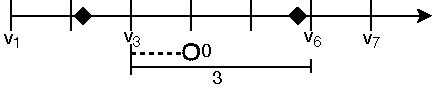
\includegraphics[width=0.7\linewidth]{img/problem.pdf}
%	\caption{Example change history of query $q_1$.}
%	\label{fig:problem}
%\end{figure}

\paragraph{Architecture:} We propose a method to predict answers for the OSC and TTL problems. Our method primarily considers static features of the query: these include statistics such as the number of triple patterns, as well as the presence of query operators, such as \texttt{UNION}, \texttt{OPTIONAL}, specific path expressions, etc.; our model can also consider statistics about predicates in the dynamic RDF graph, as well as in which past versions of the dynamic graph the results for the query changed. Figure~\ref{fig:schema} shows the components of our approach, which receives as input a SPARQL query (the architecture itself already encodes information about the dynamic graph and the value of $k$ for OSC, which we set in experiments to 1, predicting changes in the next version). The Feature Extractor decomposes the query into a set of numeric features. The Dynamics Model accepts some features of the query, as well as information from the dynamic graph, in order to compose further features. The final features are passed to a classifier in the case of the OSC problem, and to a regression model in the case of the TTL problem, to generate the final output prediction. We now describe the Feature Extractor and Dynamics Model in more detail.

\begin{figure*}[!t]
	\centering
	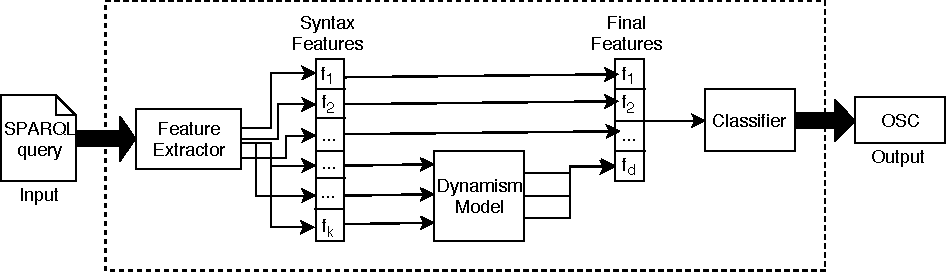
\includegraphics[width=0.9\linewidth]{img/schema.pdf}
	\caption{Proposed architecture with Feature Extractor and Dynamics Model \ah{What is $g$ here and why is it output from the Dynamics Model (rather than input)?}}
	\label{fig:schema}
\end{figure*}

\paragraph{Feature Extractor:} Our features are based on the syntactic analysis of the queries; then some features are delivered to the Dynamics Model, which provides an indicator based on the probability of change for the constant predicates within the triple patterns of the query.

We try to discover the degree of correlation between the propensity to change, with respect to numerical values, such as the number of variables, the number of triple patterns or number of predicate. We also believe that some qualitative variables may be related to the change, such as the existence of some solution-modifiers. We also consider features that describe the complexity of the queries, such as the presence of subqueries, the existence of recursive expressions in the Property Paths of the triple patterns or the existence of any type of negation.

Figure~\ref{fig:query} shows the complete list of evaluated features and shows the nominals. In the case of negation, we consider the statements MINUS, FILTER NOT EXISTS, and FILTER NOT BOUND and by the recursive path we understand those Property Paths that have patterns of the form $e*$ or $e+$ (see Definition~\ref{eq:pp}).

\begin{lstlisting}[captionpos=b, caption=Query example, label=fig:query,
basicstyle=\ttfamily,frame=single]
SELECT ?item
WHERE {
  ?item :instance_of :human .
  ?item :gender :female .
    { ?item :place_of_birth :Wales }
  UNION
    { ?item :place_of_birth ?pob .
      ?pob :located_in* :Wales }
  OPTIONAL { ?sitelink schema:about ?item .
             ?sitelink schema:inLanguage "cy" }
  FILTER (!BOUND(?sitelink))
}
LIMIT 100
\end{lstlisting}

\begin{center}
	\begin{tabular}{|l|ll|}    \hline
		1  & \# triples        & 7                             \\
		2  & \# vars           & 3                             \\
		3  & \# projected vars & 1                             \\
		4  & \# predicates     & 6                             \\
		5  & FILTER            & TRUE                          \\
		6  & LIMIT             & TRUE                          \\
		7  & UNION             & TRUE                          \\
		8  & SUBQUERY          & FALSE                         \\
		9  & *PATH             & TRUE                          \\
		10 & NEGATION          & TRUE                          \\
		11 & predicates        & {[}$p_1$,...,$p_k${]}    \\    \hline
	\end{tabular}
\end{center}



\subsection{RDF Dynamics Model}

We propose a model to estimate the dynamics of the results of a SPARQL query on an RDF dataset. The intuition behind our model is to capture how many triples change for a predicate in a time interval. For this, in the following, we define \textit{Predicate Multiplicity of an RDF dataset}.

\begin{definition}[Predicate Multiplicity of an RDF Dataset]
	Given an RDF dataset $d$ and a predicate $p$, the multiplicity of $p$ in $d$, denoted by $M(p,d)$, is:
	\begin{equation}
	\label{eq:pm}
	M(p,d) = |\{(x,y,z) \in d : y = p \}|
	\end{equation}
\end{definition}


\begin{example}
	\label{ex:pm}    
	Considering Example~\ref{ex:dataset}, the Predicate Multiplicity of predicate \textit{image} in $d_6$ dataset is:    $M(image,d_6) = 2$
\end{example}

Then, we must capture the change between two versions of an RDF dataset at the triples level, which represents triples added and deleted between the versions. For this purpose, we define a \textit{Difference Set} as an RDF dataset denoted by $\Delta(d_1, d_2)$ applying low-level change detection techniques.

\begin{definition}[Difference Set]
	Let $d_1$ and $d_2$ be two RDF datasets; a Difference Set denoted by $\Delta(d_1, d_2)$ is:
	\begin{equation}
	\label{eq:ds}
	\Delta(d_1, d_2) = \{t \mid t \in d_2 \wedge t \notin d_1\} \cup \{t \mid t \in d_1 \wedge t \notin d_2\}
	\end{equation}
\end{definition}

\begin{example}
	\label{ex:ds}
	We show the Difference Set between versions $d_1$ and $d_6$:\\
	\begin{center}    
		\begin{tabular}{lll}    \hline
			\multicolumn{3}{c}{$\Delta(d_1, d_6)$} \\    \hline
			-    :Atlantic\_Ocean  & :temperature   & 40$\degree$F          \\
			+    :Atlantic\_Ocean  & :temperature   & 60$\degree$F          \\
			+    :Atlantic\_Ocean  & :image         & AOcean2.png              \\    \hline
		\end{tabular}
	\end{center}
	
	We can now denote the Predicate Multiplicity of a Difference Set of $d_1$ and $d_2$ by $M(p, \Delta(d_1, d_2))$, e.g., $M(image, \Delta(d_1, d_6)) = 1$.
\end{example}


Following the intuition of our model, we now look for the multiplicity of a predicate $p$ of a dynamic dataset $\mathcal{D}$ in a time interval $[n,m]$.

\begin{definition}[Aggregated Predicate Multiplicity of a dynamic dataset]
	Let $\mathcal{D} = (d_1, d_2, ..., d_m)$ be a dynamic dataset, and $p$ a predicate. The Aggregated Predicate Multiplicity of $\mathcal{D}$ in a time interval $[n,m]$, denoted by $AM(p, \mathcal{D},[n,m])$ is:
	\begin{equation}
	\label{eq:apm}
	AM(p, \mathcal{D},[n,m]) = \sum_{i=n}^{m-1}M(p, \Delta(d_i, d_{i+1}))
	\end{equation}
\end{definition}

\begin{example}
	\label{ex:apm}
	$AM(temperature, \mathcal{D},[1, 7]) =$
	
	$ \sum_{i=1}^{6}M(temperature, \Delta(d_i, d_{i+1})) = 4$
	
	\begin{center}    
		\begin{tabular}{lll}    \hline
			\multicolumn{3}{c}{$\sum_{i=1}^{6}\Delta(d_i, d_{i+1})$} \\    \hline
			-    :Atlantic\_Ocean  & :temperature   & 40$\degree$F          \\
			+    :Atlantic\_Ocean  & :temperature   & 50$\degree$F          \\            
			-    :Atlantic\_Ocean  & :temperature   & 50$\degree$F          \\
			+    :Atlantic\_Ocean  & :temperature   & 60$\degree$F          \\
			+    :Atlantic\_Ocean  & :image         & AOcean2.png              \\    \hline
		\end{tabular}
	\end{center}
\end{example}

We can now denote the Aggregated Multiplicity of a dynamic dataset in a time interval $[n,m]$ by:

\begin{equation}
\label{eq:am}
AM(\mathcal{D},[n,m]) = \sum_{p \in P}AM(p, \mathcal{D},[n,m])
\end{equation}\\
Where $ P $ denotes the set of all predicates that have changed in the interval $[n,m]$.

\begin{example}
	\label{ex:am}
	$AM(\mathcal{D},[1,7]) = AM(temperature, \mathcal{D},[1,7])$
	
	$+ AM(image, \mathcal{D},[1,7]) = 5$
\end{example}

Finally, the \textit{Dynamics} of a predicate is given by the \textit{Aggregated Predicate Multiplicity of a dynamic dataset} $\mathcal{D}$ divided by \textit{Aggregated Multiplicity of a dynamic dataset}.

\begin{equation}
\label{eq:dyn}
Dyn(p, \mathcal{D},[n,m]) = \frac{AM(p, \mathcal{D},[n,m])}{AM(\mathcal{D},[n,m])}
\end{equation}

\begin{example}
	\label{ex:dyn}
	Considering our example:
	
	$ Dyn(temperature, \mathcal{D},[1,7]) = \frac{4}{5} = 0.8$
	
	$ Dyn(image, \mathcal{D},[1,7]) = \frac{1}{5} = 0.2$
	
	$ Dyn(area, \mathcal{D},[1,7]) = \frac{0}{5} = 0$
\end{example}

Considering our proposed model, the Dynamics Model component receives the set of predicates extracted from the queries, calculates the $Dyn(p, \mathcal{D},[n,m])$ for each predicate $p$ and provides the value of a Transformation Function on these indicators. The intention of the Transformation Function is to estimate the dynamics of the query based on the Dynamics of the predicates.


\section{Datasets}
\label{sec:data}

We conducted an empirical study to evaluate the effectiveness of our proposal to predict change in SPARQL query results. For this, we need an RDF dataset, with a lot of information, preferably, cross-domain, and that is constantly updated since we assume that the information of the dataset is correct, complete, but dynamic. We also need a set of queries appropriate to the chosen dataset, preferably a heterogeneous set defined by real users and covering a large part of the dataset.

\subsection{RDF Dataset}

We use 23 Wikidata snapshots from 18/04/2017 to 27/09/2017, which are captured weekly in truthy version, which represents statements that have the best non-deprecated rank for a given property. 
The first version has 1,102,242,331 triples, 57,499,191 unique IRIs, 3,276 unique predicates, 933,588,860 literals, and 7,449 blank nodes, while the final version has 1,924,967,162 triples (+74\%), 80,637,164 unique IRIs (+40\%), 3,660 unique predicates (+11\%), 1,676,930,476 literals (+79\%) and 8,909 blank nodes (+19\%). Figure~\ref{graph:datasize} shows the growth maintained over the period of some of these indicators. The gap in week 12 is due to the fact that we were not able to obtain the data for that week. Even though the information is relatively incremental, there are deletions. Figure~\ref{graph:delta} shows the ratio of triples eliminated and added each week.

\begin{figure}[h]
	\begin{minipage}[b]{0.40\linewidth}
		\centering
		\begin{tikzpicture}[thick, scale=0.5]
		\begin{axis}[
		%title={Temperature dependence of CuSO$_4\cdot$5H$_2$O solubility},
		xlabel={Version},
		ymin=0,
		xtick={0,5,10,15,20,25},
		legend pos=north west,
		ymajorgrids=true,
		grid style=dashed,
		]
		
		\addplot[
		color=blue,
		mark=square,
		]
		coordinates {
			(1,1102242331)(2,1138975810)(3,1141303957)(4,1170283653)(5,1176093821)(6,1184177503)(7,1190456714)(8,1211813217)(9,1239145151)(10,1271353260)(11,1293099057)
		};
		
		\addplot[
		color=blue,
		mark=square,
		]
		coordinates {
			(13,1348622441)(14,1418460320)(15,1432143355)(16,1470298276)(17,1506140622)(18,1542278452)(19,1593334993)(20,1613832004)(21,1684774955)(22,1771601730)(23,1843086909)(24,1924967162)
		};
		
		%\legend{# entities}
		%\legend{# predicates}
		%\legend{# literals}
		%\legend{# blank nodes}
		
		\end{axis}
		\end{tikzpicture}
		\caption{Evolution of the number of triples on Wikidata.}
		\label{graph:datasize}
	\end{minipage}
	\hspace{0.5cm}
	\begin{minipage}[b]{0.40\linewidth}
		\centering
		\begin{tikzpicture}[thick, scale=0.5]
		\begin{axis}[
		x tick label style={
			/pgf/number format/1000 sep=},
		%ylabel=\#Triples,
		enlargelimits=0.05,
		legend style={at={(0.5,-0.1)},
			anchor=north,legend columns=-1},
		ybar interval=0.7,
		]
		\addplot 
		coordinates {(1,40137188)(2,4563382)(3,29302968)(4,8906402)(5,11455047)(6,11435682)(7,27229516)(8,26968577)(9,38952400)(10,20283316)(11,0)(12,0)(13,70073220)(14,17685830)(15,45405782)(16,41199256)(17,42633484)(18,56683899)(19,25309217)(20,25030143)(21,22548371)(22,23330356)(23,37009794)};
		\addplot 
		coordinates {(1,3403743)(2,2235268)(3,1116111)(4,3096270)(5,3371448)(6,5156519)(7,5873153)(8,1336452)(9,6744349)(10,999601)(11,0)(12,0)(13,1123311)(14,4002828)(15,7250907)(16,5356971)(17,6495717)(18,5627376)(19,4812243)(20,790590)(21,681118)(22,1194899)(23,998105)};
		\legend{Added, Removed}
		\end{axis}
		\end{tikzpicture}
		\caption{Triples added and removed in Wikidata.}
		\label{graph:delta}
	\end{minipage}
\end{figure}

\subsection{Queries Dataset}

As opposed to RDF data, which can be easily obtained in the form of dumps, at the time of conducting this research, we did not find any structured dataset with queries following the Wikidata data model and Wikidata query logs where inaccessible. We considered then 388 queries of examples from Wikidata page\footnote{https://www.wikidata.org/wiki/Wikidata:SPARQL\_query\_service/queries/examples}.

Then, the queries had to be curated manually, because they had syntax errors; others asked information external to Wikidata or asked for qualifiers that are not present in the truthy version. We also eliminated the queries that returned bindings to blank nodes to facilitate the comparison between the results. Therefore, we need deterministic queries. In our case, we eliminate the queries with the keyword SAMPLE and add ORDER BY to all the queries with all the projected variables. The latter change also facilitates the detection of changes in the results. Also, we removed the use of custom Label service of Wikidata\footnote{https://www.mediawiki.org/wiki/Wikidata\_Query\_Service/User\_Manual\#Label\_service}.

Figures~\ref{fig:languageB} and \ref{fig:languageA} shows an example of several transformations of a query.

\begin{lstlisting}[captionpos=b, caption=Query transformation. Before., label=fig:languageB,
basicstyle=\ttfamily,frame=single]
#Cats
SELECT ?item ?itemLabel
WHERE {
  ?item wdt:P31 wd:Q146 .
  SERVICE wikibase:label
    { bd:serviceParam wikibase:language "en,es" }
}
\end{lstlisting}

\begin{lstlisting}[captionpos=b, caption=Query transformation. After., label=fig:languageA,
basicstyle=\ttfamily,frame=single]
#Cats
SELECT ?item ?itemLabel
WHERE {
  ?item wdt:P31 wd:Q146 .
  OPTIONAL {?item rdfs:label ?en.FILTER(LANG(?en)="en")}
  OPTIONAL {?item rdfs:label ?es.FILTER(LANG(?es)="es")}
  BIND(str(COALESCE(?en, ?es, strafter(str(?item),
    "http://www.wikidata.org/entity/"))) AS ?itemLabel)
}
ORDER BY ?item ?itemLabel
\end{lstlisting}

In the end, we have 221 curated queries. Then, we analyze the structure of the triple patterns of the queries. This is important, because our notion of freshness focuses on predicates. This restricts our approach to queries with triple patterns with a constant in the predicate position. Table~\ref{tab:Pattern} shows that in total 90.35\% of the triple patterns have a constant in the predicate position, which validate our approach of using a model based on the dynamics of predicates.

\begin{table}[h]
	\begin{minipage}[b]{0.45\linewidth}
		\caption{Triple patterns (C=Constant, V=Variable).}
		\begin{tabular}{lrr}    \hline
			Pattern & Absolute & Relative \\    \hline
			V C V   & 751      & 71.73\%    \\
			V C C   & 189      & 18.05\%    \\
			V V V   & 9        & 0.86\%     \\
			C C V   & 6        & 0.57\%     \\
			V V C   & 5        & 0.48\%     \\
			C V V   & 3        & 0.29\%     \\
			C V C   & 1        & 0.10\%      \\
			C C C   & 0        & 0.00\%        \\    \hline
			V P C   & 69       & 6.59\%     \\
			V P V   & 13       & 1.24\%     \\
			C P V   & 1        & 0.10\%      \\
			C P C   & 0        & 0.00\%        \\    \hline
		\end{tabular}
		\label{tab:Pattern}
	\end{minipage}
	\hspace{1cm}
	\begin{minipage}[b]{0.45\linewidth}
		\caption{Structure of navigational Property Paths.}
		\label{tab:Path}
		\begin{tabular}{lrr}    \hline
			Rules                & Absolute & Relative \\    \hline
			$P \rightarrow P* $   & 62       & 74.70\%     \\
			$P \rightarrow P / P$  & 56       & 67.47\%    \\
			$P \rightarrow P+ $   & 8        & 9.64\%     \\
			$P \rightarrow P \mid P$  & 6        & 7.23\%     \\
			$P \rightarrow P? $   & 6        & 7.23\%     \\
			$P \rightarrow !(P)$ & 0        & 0.00\%        \\
			$P \rightarrow C $    & 83       & 100.00\%      \\    \hline
		\end{tabular}
	\end{minipage}
\end{table}

Table~\ref{tab:Pattern} also shows that 7.93\% of triple patterns contain a Property Path in the predicate position. Then we set out to analyze these triples more deeply. Table~\ref{tab:Path} shows the frequency of occurrence of these patterns in our queries. It shows that $ P \rightarrow P * $ (74.70\%) and $ P \rightarrow P + $ (9.64\%) are often applied, which corresponds to our intuition to have a feature that indicates if there are triple patterns offering arbitrary length paths (*PATH). We should also notice that there is no negation at the level of the path. Our feature extractor is able to extract all constants of predicates within paths.

Finally, we evaluate the dynamics of the results of the queries considering Equation~\ref{eq:delta} between query results of the same query over consecutive versions of Wikidata.

Figure~\ref{graph:changeV} shows the sum of the $ \delta $ function for all the queries considering the consecutive results of each query for 23 weeks. We identify that approximately half of the results of the queries change every week.

Figure~\ref{graph:changeH} shows for each query how many changes registered over 23 weeks. We identify queries that change every week, others that never changed and a fairly uniform distribution of changes in the period.

\begin{figure}[h]
	\begin{minipage}[b]{0.40\linewidth}
		\centering
		\begin{tikzpicture}[thick, scale=0.5]
		\begin{axis}[
		%title={Temperature dependence of CuSO$_4\cdot$5H$_2$O solubility},
		xlabel={Version},
		ylabel={Changes},
		ymin=0, ymax=221,
		xtick={0,5,10,15,20,25},
		legend pos=north west,
		ymajorgrids=true,
		grid style=dashed,
		]
		
		\addplot[
		color=blue,
		mark=square,
		]
		coordinates {
			(1,115)(2,112)(3,118)(4,116)(5,121)(6,111)(7,127)(8,109)(9,118)(10,115)
		};
		
		\addplot[
		color=blue,
		mark=square,
		]
		coordinates {
			(12,105)(13,113)(14,118)(15,117)(16,111)(17,118)(18,112)(19,116)(20,106)(21,106)(22,129)
		};
		
		%\legend{# entities}
		%\legend{# predicates}
		%\legend{# literals}
		%\legend{# blank nodes}
		
		\end{axis}
		\end{tikzpicture}
		\caption{Query results changes by time.}
		\label{graph:changeV}
	\end{minipage}
	\hspace{0.7cm}
	\begin{minipage}[b]{0.40\linewidth}
		\centering
		\begin{tikzpicture}[thick, scale=0.5]
		\begin{axis}[
		%title={Temperature dependence of CuSO$_4\cdot$5H$_2$O solubility},
		xlabel={Queries},
		ymin=0,
		legend pos=north west,
		ymajorgrids=true,
		grid style=dashed,
		]
		
		\addplot[
		color=blue,
		mark=square,
		]
		coordinates {
			(1,21)(2,21)(3,21)(4,21)(5,21)(6,21)(7,21)(8,21)(9,21)(10,21)(11,21)(12,21)(13,21)(14,21)(15,21)(16,21)(17,21)(18,21)(19,21)(20,21)(21,21)(22,21)(23,21)(24,21)(25,21)(26,21)(27,21)(28,21)(29,21)(30,21)(31,21)(32,21)(33,21)(34,21)(35,21)(36,21)(37,21)(38,21)(39,21)(40,21)(41,21)(42,21)(43,21)(44,21)(45,20)(46,20)(47,20)(48,20)(49,20)(50,20)(51,20)(52,19)(53,19)(54,19)(55,19)(56,19)(57,19)(58,19)(59,19)(60,18)(61,18)(62,18)(63,18)(64,18)(65,18)(66,18)(67,17)(68,17)(69,17)(70,17)(71,17)(72,17)(73,17)(74,16)(75,16)(76,16)(77,16)(78,16)(79,16)(80,15)(81,15)(82,15)(83,15)(84,14)(85,14)(86,14)(87,14)(88,14)(89,14)(90,14)(91,14)(92,14)(93,13)(94,13)(95,13)(96,13)(97,13)(98,13)(99,12)(100,12)(101,12)(102,12)(103,12)(104,12)(105,12)(106,12)(107,12)(108,12)(109,11)(110,11)(111,11)(112,11)(113,10)(114,10)(115,10)(116,10)(117,10)(118,9)(119,9)(120,9)(121,9)(122,9)(123,9)(124,9)(125,9)(126,8)(127,8)(128,8)(129,8)(130,8)(131,8)(132,8)(133,8)(134,8)(135,8)(136,7)(137,7)(138,7)(139,7)(140,7)(141,7)(142,7)(143,6)(144,6)(145,6)(146,6)(147,6)(148,6)(149,6)(150,6)(151,5)(152,5)(153,5)(154,4)(155,4)(156,4)(157,4)(158,4)(159,4)(160,4)(161,4)(162,4)(163,4)(164,4)(165,4)(166,3)(167,3)(168,3)(169,3)(170,3)(171,3)(172,2)(173,2)(174,2)(175,2)(176,2)(177,2)(178,2)(179,2)(180,2)(181,2)(182,2)(183,2)(184,2)(185,2)(186,2)(187,2)(188,1)(189,1)(190,1)(191,1)(192,1)(193,1)(194,1)(195,1)(196,1)(197,1)(198,1)(199,1)(200,1)(201,1)(202,1)(203,1)(204,0)(205,0)(206,0)(207,0)(208,0)(209,0)(210,0)(211,0)(212,0)(213,0)(214,0)(215,0)(216,0)(217,0)(218,0)(219,0)(220,0)(221,0)
		};
		
		%\legend{# entities}
		%\legend{# predicates}
		%\legend{# literals}
		%\legend{# blank nodes}
		
		\end{axis}
		\end{tikzpicture}
		\caption{Query results changes by queries.}
		\label{graph:changeH}
	\end{minipage}
\end{figure}


\section{Evaluation}
\label{sec:eval}

We evaluate the performance of our proposal to predict changes in the results of our queries. For this, we use the Wikidata dataset and our query dataset explained previously.
To build the Difference Sets ($\Delta$) for our model we used an approach based on a merge-sort to scan over the snapshots as follows:

\begin{enumerate}
	\item Sort all statements by their syntactic order (subject-predicate-object).
	\item Perform a pairwise comparison of the statements by scanning two snapshots in linear time.
	\item Trigger a detection of the change as soon as the order of the statements differs between two snapshots.
\end{enumerate}

Then we configure the parameters of our model. For the time interval, we consider three versions of the dataset equivalent to the last three weeks. As the Transformation Function, we evaluate three basic functions: Maximum, Minimum, and Average. For example, Maximum will take the dynamics of the most dynamic property (used as a predicate in the query) as a feature.
In addition, given that existing approaches are based on the historical results of the queries, we evaluate the substitution of our model for a historical change indicator that counts how many times the results have changed in the last three weeks.

In addition, we train a Machine Learning model to determine the life spam of a query results. To train the model we consider the changes observed in the monitored interval. For each update of the results of a query, we have created an example of training with the previously presented features. The target TTL value that we learn is the time interval during which the results of the query remain fresh from the current update time.

\subsection{Results}

First, we consider the Pearson correlation between the characteristics. We found only a couple of highly correlated variables (\# triples and \# vars: 0.943). The influence of the use of various Transformation Functions in our model was also evaluated. In this case, Average was the Transformation Function that obtained the best result followed by Maximum.

We tested a list of classifiers, including Decision Tree, Nearest Neighbors, and Naive Bayes among others listed in Table~\ref{tab:classifier}. Our pilot experiment shows that Nearest Neighbors and Decision Tree work better than the others. We evaluated the quality of our proposal by forming a set of classifiers to predict the change of 221 queries in 15 weeks, which is equivalent to 3315 objects to classify, described in terms of our proposed features. We split the data 80\% for training and 20\% for tests. To avoid overfitting, we use cross-validation in the training data.

Table~\ref{tab:classifier} shows the quality values of the classifiers evaluated in terms of $F_1$. To have a measure of the positioning of our proposal, we added a new feature that counts how many times the results of the query change on average in the last three versions. Then, we did two executions with our syntactic features: one using this new indicator, and the second with our dynamic model. Table~\ref{tab:classifier} shows that our algorithm achieved less quality. Despite obtaining lower results, the quality of our proposal is not far from that achieved by observing the results of queries in the past, but certainly, our approach is less expensive since it does not require knowledge of past query results.

Finally, to predict the time that the results of a query will remain invariant (TTL), a continuous value (number of weeks) will be determined. For that we employed techniques of multiple linear regression using the sklearn and tensorflow library. The latter allows us to see how the periods of estimation and the convergence analysis will behave.

We were able to predict the time of life (in relation to the number of invariant weeks) with an average square error of 0.43 and a variance score of 0.01. These results allow to predict future changes in query results with good accuracy using linear regression techniques.


\begin{table*}[h]
	\centering
	\caption{Tested classifiers.}
	\label{tab:classifier}
	\begin{tabular}{|l|r|r|}    \hline		
		Classifier                   & Past Results & Dynamics Model \\    \hline
		Base Dummy 					 & 0.497869 & 0.486923 \\
		Nearest Neighbors            & 0.701587 & 0.635923 \\
		Decision Tree                & 0.695591 & 0.651462 \\
		Linear SVM                   & 0.705755 & 0.593846 \\
		Naive Bayes                  & 0.661239 & 0.587692 \\    \hline
	\end{tabular}
\end{table*}
\begin{comment}

\begin{figure}
	\centering
	\begin{tikzpicture}[thick, scale=1]
	\begin{axis}
	
	\addplot 
	coordinates {("Base Dummy",40137188)("Nearest Neighbors",4563382)("Decision Tree",29302968)("Linear SVM",8906402)("Naive Bayes",11455047)};
	\addplot 
	coordinates {(Base Dummy,40137188)(Nearest Neighbors,4563382)(Decision Tree,29302968)(Linear SVM,8906402)(Naive Bayes,11455047)};
	\legend{Added, Removed}
	\end{axis}
	\end{tikzpicture}
	\caption{Triples added and removed in Wikidata.}
	\label{graph:delta}
\end{figure}
\end{comment}


\section{Conclusion and Future Work}
\label{sec:conclusion}

In this paper we propose classifiers that predict whether or not the results of a query will change in the short time interval; for this, we propose a model based on the dynamics of the predicates in the datasets and a set of features extracted from the syntax of the queries. The proposed framework is flexible for incorporating new features extracted from the queries, from the current results, or from the model based on the multiplicity of predicates.

We select the datasets to evaluate our proposal considering desirable characteristics, such as availability, size, dynamics, and integrity. Choosing Wikidata, we present statistics to understand such characteristics. In the case of the queries dataset, we did not find any existing dataset of queries that complied with the requirements, so we curated a query dataset for Wikidata based on query examples proposed by users.

Finally, we evaluate our proposal, making a weekly prediction of change in the results of the queries and evaluating the success rates of the different classifiers each week based on F-measure. We also apply linear regression techniques to predict, specifically, when the results of a query will change.
We measure the effectiveness of the characteristic based on our model of predicate dynamics versus a characterization of dynamics based on the historical results. The latter is a common factor in the previous proposals, but it requires a high cost. Our results show that our approach using predicate dynamics is competitive for prediction while being less expensive to support.    

Although the results obtained are encouraging, they are still preliminary. We consider for future work evaluating the quality of our proposal over a longer period. In addition, we believe that more complex query features can improve the results, such as considering operator semantics; for example, to see if negation is affecting predicates or if the predicates are affected by the existence of filters. On the other hand, it would be worth expanding the set of queries in the test dataset, in order to increase the size, complexity, and coverage. Recently a query dataset for Wikidata was published\footnote{https://lists.w3.org/Archives/Public/semantic-web/2018Aug/0023.html}. It would be good to evaluate this query dataset, as well as consider a probabilistic approach based on query algebra (rather than syntax).


\bibliographystyle{splncs04}
\bibliography{ref}

\end{document}
